\chapter{Использование кольцевого развязанного делителя мощности}

Поисследуем кольцевой развязанный делитель мощности в роли устройства сложения сигналов.

\section{Исследование разбаланса амплитуд}

Подавать сигналы будем с портов типа \code{P\_1Tone}, для первой прикидки по 10 дБмВт без сдвига по фазе.
Задавать входные сигналы будем с помощью переменных $P_\text{in1} = P_\text{in2} = polar(dbmtow(10), 0)$.
В дальнейшем при исследовании будем менять только эти переменные.
Общий вид моделируемой схемы можно увидеть на Рис.~\ref{fig:afd_homework_4_schematic}

\begin{figure}[!ht]
    \centering
    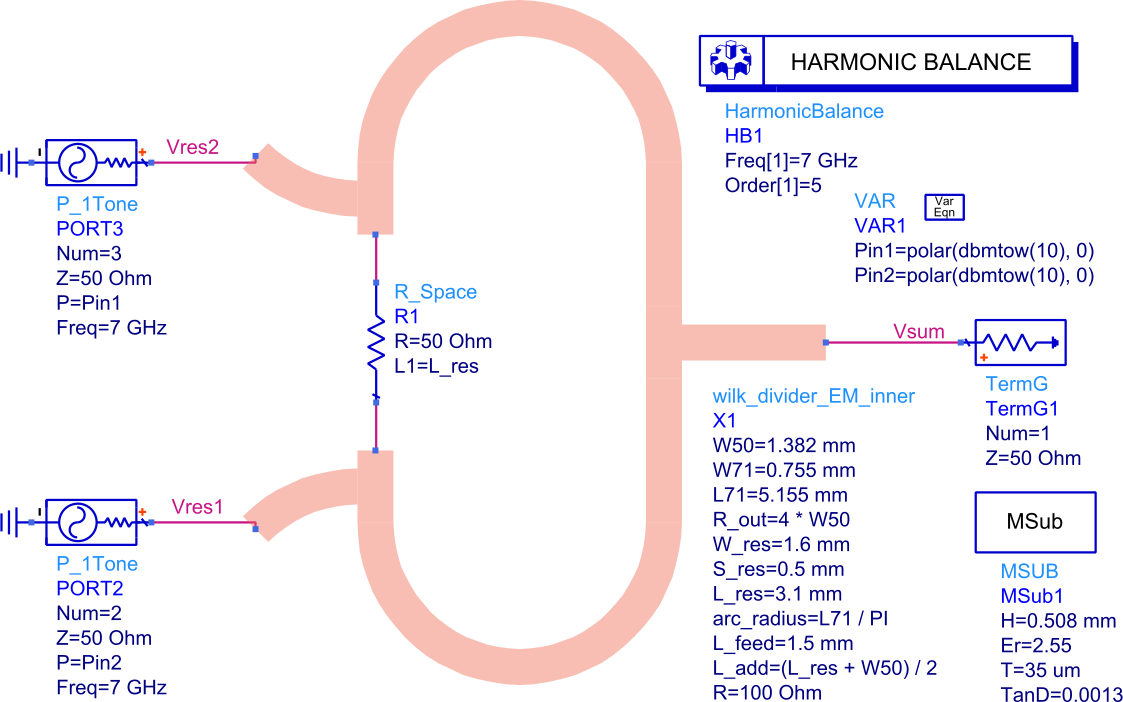
\includegraphics[width=0.8\textwidth]{afd_homework_4_schematic.pdf}
    \caption{Моделируемая схема}%
    \label{fig:afd_homework_4_schematic}
\end{figure}

Для определения мощности, рассеиваемой на резисторе, нужно знать падение напряжения на нем и ток, протекающий через него.
Для передачи в датасет значений токов, протекающих через резистор, добавим токи, протекающие через выходы резистора.

По результатам моделирования рассчитаем рассеиваемую на резисторе мощность, для чего воспользуемся выражениями, представленными на Рис.~\ref{fig:afd_homework_4_data_1_equations}.

\begin{figure}[!ht]
    \centering
    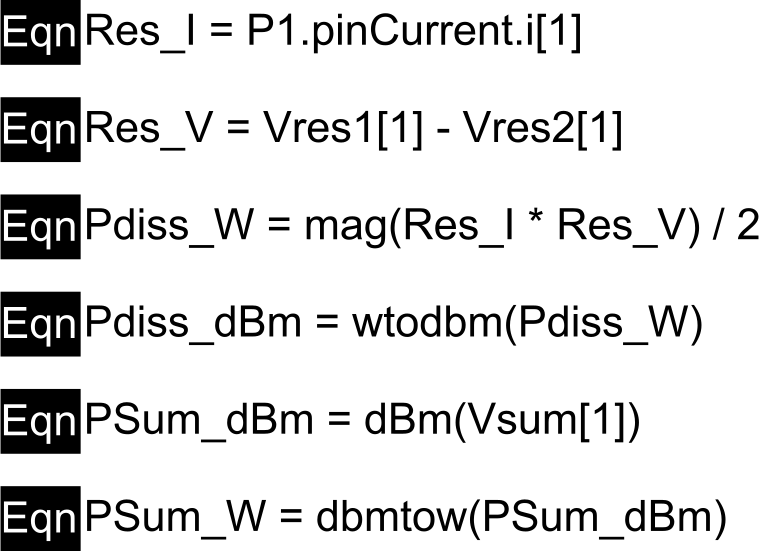
\includegraphics[width=0.4\textwidth]{afd_homework_4_data_1_equations.pdf}
    \caption{}%
    \label{fig:afd_homework_4_data_1_equations}
\end{figure}

Видно, что при симметричных сигналах практически вся мощность идет на выход и ничего не рассеивается на развязывающем резисторе (Рис.~\ref{fig:afd_homework_4_data_1_balanced_table}).

\begin{figure}[!ht]
    \centering
    \includegraphics[width=0.6\textwidth]{afd_homework_4_data_1_balanced_table.pdf}
    \caption{}%
    \label{fig:afd_homework_4_data_1_balanced_table}
\end{figure}

Введем разбаланс амплитуд.
Уменьшим мощность на одном из каналов в два раза ($P_\text{in2} = 7~\text{дБм}$).
Результат представлен на Рис.~\ref{fig:afd_homework_4_data_1_amplitudes_diff_3_dBm_table}.

\begin{figure}[!ht]
    \centering
    \includegraphics[width=0.6\textwidth]{afd_homework_4_data_1_amplitudes_diff_3_dBm_table.pdf}
    \caption{}%
    \label{fig:afd_homework_4_data_1_amplitudes_diff_3_dBm_table}
\end{figure}

Видно, что суммарная выходная мощность $14.5~\text{мВт}$ незначительно отличается от суммы входных мощностей, равной $15~\text{мВт}$, но появилось незначительное рассеяние мощности на резисторе, равное $600~\text{мкВт}$.

Пусть разбаланс амплитуд будет теперь таким, чтоб мощность на втором канале была в 10 раз меньше, чем на первом ($P_{in2} = 0~\text{дБм}$).
Результат представлен на Рис.~\ref{fig:afd_homework_4_data_1_amplitudes_diff_10_dBm_table}.

\begin{figure}[!ht]
    \centering
    \includegraphics[width=0.6\textwidth]{afd_homework_4_data_1_amplitudes_diff_10_dBm_table.pdf}
    \caption{}%
    \label{fig:afd_homework_4_data_1_amplitudes_diff_10_dBm_table}
\end{figure}

Теперь суммарная выходная мощность, равная $8.6~\text{мВт}$ становиться меньше мощности суммы мощностей на каждом канале в отдельности.
На резисторе, тем временем, рассеивается порядка $4~\text{мВт}$.

Окончательно отключим один канал ($P_{in2} = 0$).
Результат представлен на Рис.~\ref{fig:afd_homework_4_data_1_amplitudes_diff_inf_dBm_table}.

\begin{figure}[!ht]
    \centering
    \includegraphics[width=0.6\textwidth]{afd_homework_4_data_1_amplitudes_diff_inf_dBm_table.pdf}
    \caption{}%
    \label{fig:afd_homework_4_data_1_amplitudes_diff_inf_dBm_table}
\end{figure}

Выходная мощность равна половине входной мощности от первого канала, при этом вторая половина рассеивается на резисторе.

\section{Исследование разбаланса фаз}

Исследуем влияние разбаланса фаз при суммировании равных мощностей.
Пусть на входы приходят два сигнала по $1~\text{Вт}$ с разностью фаз $30°$.
Результат представлен на Рис.~\ref{fig:afd_homework_4_data_1_phase_diff_30_table}.

\begin{figure}[!ht]
    \centering
    \includegraphics[width=0.6\textwidth]{afd_homework_4_data_1_phase_diff_30_table.pdf}
    \caption{}%
    \label{fig:afd_homework_4_data_1_phase_diff_30_table}
\end{figure}

Суммарная выходная мощность, равная $1.86~\text{Вт}$ меньше суммы входных мощностей.
Часть мощности рассеивается на резисторе.

Установим разбаланс фаз в $60°$.
Результат представлен на Рис.~\ref{fig:afd_homework_4_data_1_phase_diff_60_table}.

\begin{figure}[!ht]
    \centering
    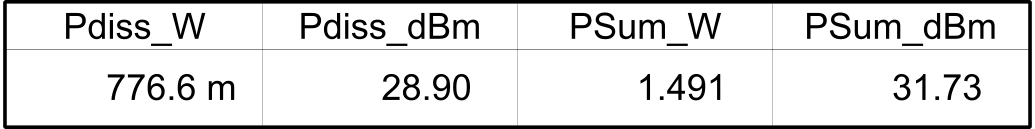
\includegraphics[width=0.6\textwidth]{afd_homework_4_data_1_phase_diff_60_table.pdf}
    \caption{}%
    \label{fig:afd_homework_4_data_1_phase_diff_60_table}
\end{figure}

Суммарная выходная мощность, равная $1.5~\text{мВт}$, меньше суммы входных мощностей.
Больше трети от суммы входных мощностей рассеивается на резисторе.

Установим разбаланс фаз в $90°$.
Результат представлен на Рис.~\ref{fig:afd_homework_4_data_1_phase_diff_90_table}.

\begin{figure}[!ht]
    \centering
    \includegraphics[width=0.6\textwidth]{afd_homework_4_data_1_phase_diff_90_table.pdf}
    \caption{}%
    \label{fig:afd_homework_4_data_1_phase_diff_90_table}
\end{figure}

Суммарная выходная мощность, равная $1~\text{Вт}$, меньше суммы входных мощностей и, более того, не превышает мощность какого-либо из каналов в отдельности.
Половина суммы входных мощностей рассеивается на резисторе.

Окончательно установим входные сигналы противофазными.
Результат представлен на Рис.~\ref{fig:afd_homework_4_data_1_phase_diff_180_table}.

\begin{figure}[!ht]
    \centering
    \includegraphics[width=0.6\textwidth]{afd_homework_4_data_1_phase_diff_180_table.pdf}
    \caption{}%
    \label{fig:afd_homework_4_data_1_phase_diff_180_table}
\end{figure}

Вся сумма входных мощностей рассеивается на резисторе, на выход не идет ничего.

Также при проведении таких исследований нужно смотреть, хватает ли способности использованного типоразмера резистора для рассеивания выделяемой на нем мощности.
При превышении этого параметра резистор может легко сгореть и повредить аппаратуру.
В моделируемом делителе использован резистор типоразмера 1206, способный рассеивать до $63~\text{мВт}$.

Видно, что для исследованных значений разбалансов амплитуд развязывающего резистора хватает.
А вот при подаче двух сигналов мощностью в $1~\text{Вт}$ с разбалансом фаз уже в $30°$ этого резистора уже не хватит для рассеивания мощности, приходящейся на него.

Таким образом, можно сделать вывод, что моделируемый кольцевой развязанный делитель хорошо подходит для сложения синфазных сигналов равных амплитуд и устойчив к большому диапазону разбалансировки амплитуд при разумном абсолютном значении последних, однако даже небольшой разбаланс фаз способен вывести его из строя даже при достаточно малых амплитудах.
